
\begin{problem}{Search Again}

Consider the state space graph shown below.  A is the start state and
G is the goal state. The costs for each edge are shown on the graph.
Each edge can be traversed in both directions.

\begin{center}
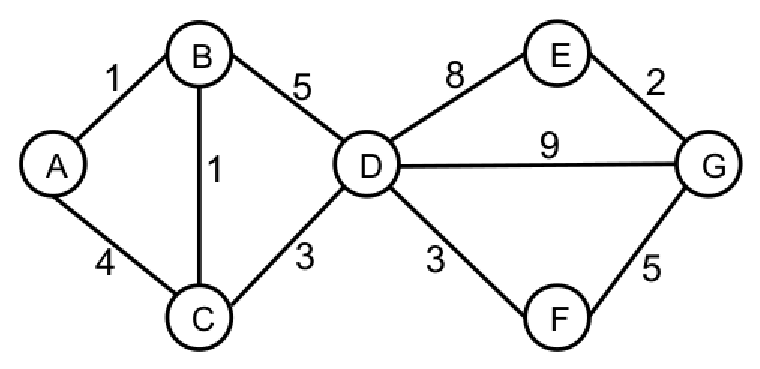
\includegraphics[width=3.5in]{figures/search_graph.eps}
\end{center}

\textbf{Use the Graph Search Algorithm (v2) discussed in class.}
Execute the following search algorithms using priority queues, by
filling in the search table for each part. Write nodes as a tuple containing a state sequence and cost (e.g. (A-B-C, 2)). Note that for Breadth first and Depth first the algorithms ignore the true "cost" so you can just use the depth of the node as the second part of the tuple and then expand nodes with either the highest or lowest depth. Break ties alphabetically.  Note that all steps in the table below will not
necessarily be used. You may skip any steps where a node is removed from the frontier but not expanded. Note that nodes are only expanded after they are removed from the frontier, after checking the goal test, and after checking if not in the closed set.

    
\begin{question}[3]
Breadth First Graph Search

    \begin{tabular}{|l|l@{\hspace*{4.5in}}|l|} \hline
    \bf Step & \bf Priority Queue                                   & \bf Expand \\ \hline
    1 &      \fiveai                                                       & \fiveaib \\ \hline
    2 &     \fiveaii                                                            & \fiveaiib \\ \hline
    3 &    \fiveaiii                                                         & \fiveaiiib \\ \hline
    4 &    \fiveaiv                                                         & \fiveaivb \\ \hline
    5 &      \fiveav                                                       &  \\ \hline
    6 &   \fiveavi                                                          & \fiveavib \\ \hline
    7 &    \fiveavii                                                         & \fiveaviib \\ \hline
    8 &   \fiveaviii                                                          & \fiveaviiib \\ \hline
    \end{tabular}

    Solution: \fivea

\end{question}

\begin{question}[3]
Depth First Graph Search.\\
    \begin{tabular}{|l|l@{\hspace*{4.5in}}|l|} \hline
    \bf Step & \bf Priority Queue                                   & \bf Expand \\ \hline
    1 &      \fivebi                                                       & \fivebib \\ \hline
    2 &     \fivebii                                                            & \fivebiib \\ \hline
    3 &    \fivebiii                                                         & \fivebiiib \\ \hline
    4 &    \fivebiv                                                         & \fivebivb \\ \hline
    5 &      \fivebv                                                       &  \\ \hline
    6 &   \fivebvi                                                          & \fivebvib \\ \hline
    7 &    \fivebvii                                                         & \fivebviib \\ \hline
    8 &   \fivebviii                                                          & \fivebviiib \\ \hline
    \end{tabular}

    Solution:\fiveb
\end{question}

\newpage
\begin{question}[3] 
Uniform Cost Graph Search. \\

    \begin{tabular}{|l|l@{\hspace*{4.5in}}|l|} \hline
    \bf Step & \bf Priority Queue                                   & \bf Expand \\ \hline
    1 &      \fiveci                                                       & \fivecib \\ \hline
    2 &     \fivecii                                                            & \fiveciib \\ \hline
    3 &    \fiveciii                                                         & \fiveciiib \\ \hline
    4 &    \fiveciv                                                         & \fivecivb \\ \hline
    5 &      \fivecv                                                       &  \\ \hline
    6 &   \fivecvi                                                          & \fivecvib \\ \hline
    7 &    \fivecvii                                                         & \fivecviib \\ \hline
    8 &   \fivecviii                                                          & \fivecviiib \\ \hline
    \end{tabular}

    Solution:\fivec


\end{question}

\begin{question}
Heuristic Search

 \begin{subquestion}[4] Consider the two heurisitics $h_1$ and $h_2$, only one of
     which is consistent.  Which one is consistent?

     \fivedh

\end{subquestion}

\begin{center}
\begin{tabular}{|c|c|c|c|c|c|c|c|}\hline
Node  & A   & B  & C  & D  & E   & F   & G  \\ \hline
$h_1$ & 9.5 & 9	 & 8  & 7  & 1.5 & 4   & 0  \\ \hline
$h_2$ & 10  & 12 & 10 & 8  & 1   & 4.5 & 0  \\ \hline
\end{tabular}
\end{center}
\begin{subquestion}[3]
Then do A* search with that heuristic.

    \begin{tabular}{|l|l@{\hspace*{4.5in}}|l|} \hline
    \bf Step & \bf Priority Queue                                   & \bf Expand \\ \hline
    1 &      \fivedi                                                       & \fivedib \\ \hline
    2 &     \fivedii                                                            & \fivediib \\ \hline
    3 &    \fivediii                                                         & \fivediiib \\ \hline
    4 &    \fivediv                                                         & \fivedivb \\ \hline
    5 &      \fivedv                                                       &  \\ \hline
    6 &   \fivedvi                                                          & \fivedvib \\ \hline
    7 &    \fivedvii                                                         & \fivedviib \\ \hline
    8 &   \fivedviii                                                          & \fivedviiib \\ \hline
    \end{tabular}

    Solution: \fived
\end{subquestion}

 \begin{subquestion}[9]
 Suppose you are completing the new heuristic function $h_3$
    shown below.  All the values are fixed except $h_3(B)$.

\begin{center}
\begin{tabular}{|c|c|c|c|c|c|c|c|}
\hline
Node & A & B & C & D & E & F & G \\
\hline
$h_3$& 10 & ?  & 9 & 7 & 1.5 & 4.5& 0 \\
\hline
\end{tabular}
\end{center}

For each of the following conditions, write the set of values that are
possible for $h_3(B)$.  For example, to denote all non-negative
numbers, write [0, $\infty$], to denote the empty set, write
$\emptyset$, and so on.

\begin{enumerate}

\item What values of $h_3(B)$ make $h_3$ admissible?

\fivelasta

\item What values of $h_3(B)$ make $h_3$ consistent?


\fivelastb

\item What values of $h_3(B)$ will cause A* graph search to expand
  from node A to C, then node A to B, then node A to B to D in that
  order?

\fivelastc

\end{enumerate}

\end{subquestion}

\end{question}

\end{problem}